\chapter{Deep Learning Basics}
\label{ch:deep-learning-basics}

This chapter introduces some basic concepts about deep learning. Deep learning covers a large spectrum of applications. Categorized by the type of input data, deep learning models can be roughly classified into two classes --- \emph{feedforward neural network} for non-sequential data, such as static images, and \emph{recurrent neural network} for sequential data, such as video, audio, or text in natural language. Deep learning also belongs to general machine learning, therefore multiple frameworks have been developed to adopt different levels of supervisory signals, including supervised, semi-supervised, unsupervised, and reinforcement learning. In this chapter we focus on the supervised learning of feedforward neural networks, which is also mainly used in this dissertation.

For supervised learning, a training dataset can be denoted by $\mathcal{D}_{train}=\left\{(x^{(i)}, t^{(i)})\right\}_N$, where $x$ and $t$ are input and target tensor, respectively, and $N$ is the number of samples. A feedforward neural network is a parameterized function $f_\theta(x)$ that maps an input $x$ to some output tensor $y$. The learning objective is to find the best parameter $\theta^*$ that minimizes a predefined loss function $L(y,t)$, formally
\begin{equation} \label{eq:objfunc}
  \theta^* = \argmin_\theta \frac{1}{N} \sum_{i=1}^N L\left(f_\theta(x^{(i)}), t^{(i)}\right).
\end{equation}

Section~\ref{sec:dl-feedforward} will detail on how to parameterize $f_\theta(\cdot)$. Section~\ref{sec:dl-loss} will introduce several commonly used loss functions $L(\cdot,\cdot)$. The optimization process of finding $\theta^*$ will be elaborated in Section~\ref{sec:dl-bp}.

% Feedforward Neural Network
%   Linear Operators: FC, Conv
%   Non-linear Operators: ReLU, Softmax
%   Normalizations: Batch normalization
%   Popular networks


% Loss functions
%   Categorical
%   Regression

% Backpropagation
%   Chain Rule for DAG
%   Jacobian for stacked layers
%   Stochastic Gradient Descent

\section{Feedforward Neural Network} % (fold)
\label{sec:dl-feedforward}
A typical feedforward neural network is a sequence of linear and non-linear operators, as depicted in Figure~\ref{fig:dl-feedforward}. These linear and non-linear operators are often encapsulated into \emph{layers} when designing neural networks. The output of the previous layer is served as the input of the next layer. Below we will introduce some commonly used operators.
\begin{figure}[t]
\begin{center}
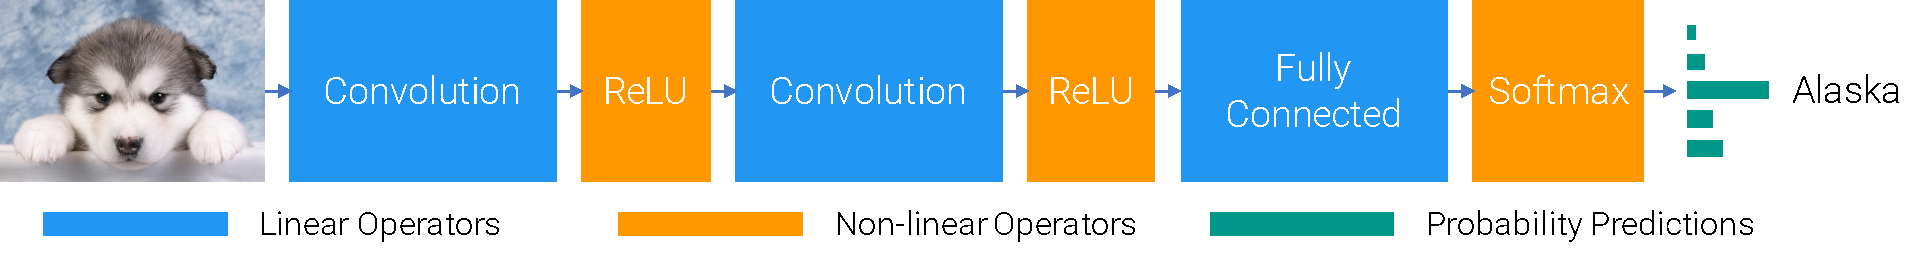
\includegraphics[width=1.0\linewidth]{figures/feedforward.pdf}
\caption{Feedforward neural network consisting of sequential linear and non-linear operators}
\label{fig:dl-feedforward}
\end{center}
\end{figure}

\subsection{Linear Operators} % (fold)
\label{sub:dl-linops}
One of the basic linear operators is matrix-vector multiplication, namely the \emph{fully connected (FC)} layer in neural network. Formally, the output of the FC layer is
\begin{equation}
  y=Wx+b,
\end{equation}
where $x\in\mathbb{R}^d$ is an input vector, $W\in\mathbb{R}^{m\times d}$ is a parameter dubbed \emph{weight} matrix, and $b\in\mathbb{R}^m$ is a parameter dubbed \emph{bias} vector. FC layers are often used as linear classifiers at then end of a neural network.

While each output dimension $y_i$, also called \emph{unit}, is computed from all of the input dimensions, sometimes people wish to constrain the size of this input range, which forms another linear operator --- \emph{convolution}. Take as an example of 3-D input image $x\in\mathbb{R}^{C\times H\times W}$ with $C$ channels and spatial size $H\times W$, a convolution layer is parameterized by $M$ convolution kernels each has a weight $w\in\mathbb{R}^{C\times (2K+1)\times (2K+1)}$ and a bias $b$, where $2K+1$ is called the kernel size (here we assume the kernel size is odd for simplicity). Applying each convolution kernel $w$ to $x$ results in an output \emph{feature map} $y\in\mathbb{R}^{H\times W}$, where
\begin{equation}
  y(i,j) = b + \sum_{c=1}^C \sum_{p=-K}^K \sum_{q=-K}^K w(c,p,q) x(c,i+p,j+q).
\end{equation}

This process is demonstrated in Figure~\ref{fig:dl-conv}. Each output unit can be seen as the inner-product between the kernel weight and the input content inside a local region, which represents their matching similarities. The convolution kernel is shared across all the output units on the feature map. Thus it serves as a pattern \emph{detector} that finds certain pattern on the input image.
\begin{figure}[t]
\begin{center}
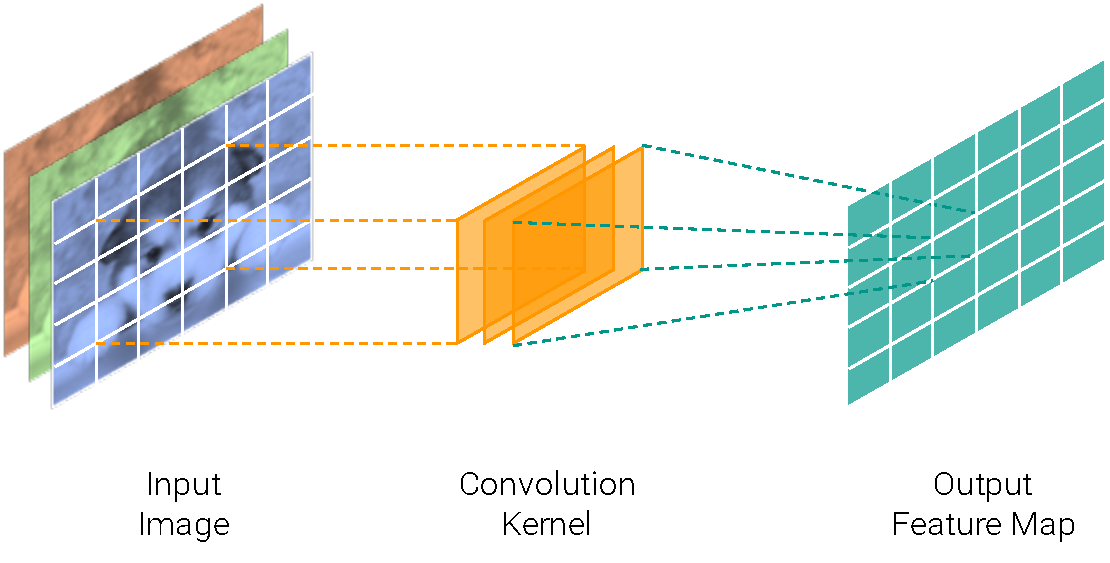
\includegraphics[width=1.0\linewidth]{figures/convolution.pdf}
\caption{Convolution operator on a 3-channel input image}
\label{fig:dl-conv}
\end{center}
\end{figure}
% subsection dl-linops (end)

\subsection{Non-linear Operators} % (fold)
\label{sub:dl-nonlinops}
Performing linear operations consecutively is useless, since they can be replaced by a single linear operation. For example, applying two FC layers
\begin{equation}
  W_2(W_1x+b_1)+b_2 = (W_2W_1)x +(W_2b_1+b_2)
\end{equation}
is equivalent to a single FC layer with parameters $(W_2W_1, W_2b_1+b_2)$. In order to enrich the function family that neural networks can represent, people often insert non-linear operators between every two linear operators.

One of the most widely used non-linear operators is \emph{rectified linear unit (ReLU)}, mathematically it is a piece-wise linear transformation applying to each input unit independently
\begin{equation}
  \mathrm{ReLU}(x) = \begin{cases}
    x & \text{when }x \ge 0,\\
    0 & \text{when }x < 0.
  \end{cases}
\end{equation}

Another common non-linear operator is \emph{softmax}, which maps a vector $x\in\mathbb{R}^d$ to a multinomial distribution
\begin{equation} \label{eq:softmax}
  y_i=\mathrm{softmax}(x)_i=\frac{\exp(x_i)}{\sum_{j=1}^d \exp(x_j)}.
\end{equation}
Note that $y_i > 0$ and $\sum_{i=1}^d y_i = 1$. It is often used at the end of a neural network for image classification, which casts the network output to a categorical distribution over predefined classes.
% subsection dl-nonlinops (end)

\subsection{Normalizations} % (fold)
\label{sub:dl-normalizations}
Normalizations form another important bunch of operators. They keep the output of each layer in a certain range of values, and ease the parameter optimization process. One of the most effective normalization operators is \emph{Batch Normalization (BN)}~\cite{ioffe2015batch}. Given $N$ input samples each denoted by a vector $x^{(i)}\in\mathbb{R}^d, i=1,\dots,N$, BN computes the mean and variance of each dimension independently across all the samples
\begin{align}
  \mu_j &= \frac{1}{N} \sum_{i=1}^N x_j^{(i)},\\
  \sigma_j^2 &= \frac{1}{N} \sum_{i=1}^N (x_j^{(i)} - \mu_j)^2.
\end{align}
Then it normalizes the input to be zero mean and unit variance by
\begin{equation}
  \hat{x}_j^{(i)} = \frac{x_j^{(i)} - \mu_j}{\sqrt{\sigma_j^2 + \epsilon}},
\end{equation}
where $\epsilon$ is a small positive number that avoids zero division. At last, BN applies a linear transformation to $\hat{x}$ by
\begin{equation}
  y_j^{(i)} = \alpha_j \hat{x}_j^{(i)} + \beta_j,
\end{equation}
where $\alpha,\beta\in\mathbb{R}^d$ are learnable parameters.
% subsection dl-normalizations (end)

\subsection{Residual Module} % (fold)
\label{sub:dl-residual}
Many popular \emph{convolutional neural network (CNNs)} have been proposed~\cite{krizhevsky2012imagenet,simonyan2014very,szegedy2014going} to tackle the image classification problem. One simple yet effective variant worth mention here is the residual module~\cite{he2015deep}. The output of this module is
\begin{equation}
  y = f_\theta(x) + x,
\end{equation}
where the parameterized function $f_\theta(\cdot)$ learns some additive residual to the input. This residual module can at least keep the input unchanged, thus it will not be worse when stacking more such layers. We refer the readers to~\cite{he2015deep,he2016identity} for more detailed benefits.
% subsection dl-residual (end)
% section dl-feedforward (end)

\section{Loss Functions} % (fold)
\label{sec:dl-loss}
\emph{Discriminative} learning has two types of objectives --- \emph{classification} and \emph{regression}. Take as an example of predicting a person's age according to his/her photo, classification predicts a categorical class, such as child, teen, middle age, or elder, while regression directly predicts the number, such as $26.5$-year old.

For classification, the target is denoted by an one-hot vector $t\in\mathbb{R}^d$ over $d$ predefined classes, where $t_i=1$ if the target is the class-$i$ and all the other dimensions are zero. The neural network usually outputs a multinomial random variable $y\in\mathbb{R}^d$ as Eq.~\eqref{eq:softmax}, and the \emph{cross entropy} loss function is often used to indicate the discrepancy between random variables $t$ and $y$:
\begin{equation}
  \mathrm{cross\ entropy}(t, y) = -\sum_{i=1}^d t_i \log y_i.
\end{equation}

For regression, both the target and the network output can be denoted by arbitrary vectors $t, y\in\mathbb{R}^d$. Different distance metrics could be used as the loss function, and the \emph{squared L2} distance is one the most widely used
\begin{equation}
  \mathrm{squared}_{L_2}(t, y) = ||t-y||_2^2 = \sum_{i=1}^d (t_i - y_i)^2.
\end{equation}
In order to improve the robustness to the outliers, Girshick \etal~\cite{girshick2015fast} proposed an alternative \emph{smooth L1} loss
\begin{equation}
  \mathrm{smooth}_{L_1}(t, y) = \sum_{i=1}^d \begin{dcases}
    0.5(t_i - y_i)^2 & \text{if }|t_i-y_i| < 1,\\
    |t_i-y_i| - 0.5  & \text{otherwise}.
  \end{dcases}
\end{equation}

% section dl-loss (end)

\section{Backpropagation} % (fold)
\label{sec:dl-bp}
Due to the highly non-linearity nature of the parametric form of a deep neural network, the objective function Eq.~\eqref{eq:objfunc} usually does not have a closed-form global optimum. Therefore, we often seek for a local optimum instead by solving Eq.~\eqref{eq:objfunc} iteratively using \emph{stochastic gradient descent (SGD)}. During each iteration, we first randomly choose a subset, which is called a \emph{minibatch} $\mathcal{D}_{minibatch} = \left\{\left(x^{(i)}, t^{(i)}\right)\right\}_M$, from the whole training set. Then we compute the gradient of the loss function \wrt the parameters
\begin{equation} \label{eq:grad}
  \nabla_\theta L = \frac{1}{M} \sum_{i=1}^M \frac{\partial L\left(f_\theta(x^{(i)}), t^{(i)}\right)}{\partial \theta},
\end{equation}
and update the parameters with a step along the direction of steepest descent
\begin{equation}
  \theta \gets \theta - \gamma \nabla_\theta L,
\end{equation}
where $\gamma$ is a scalar \emph{learning rate}.

\emph{Backpropgation (BP)}, proposed by Rumelhart~\cite{rumelhart1986learning} and LeCun~\cite{lecun1989backpropagation}, is an efficient algorithm that computes the partial gradient in Eq.~\eqref{eq:grad} efficiently, based on the \emph{chain rule} of compound functions.

\subsection{On a Chain of Layers} % (fold)
\label{sub:dl-bp-on-chain}
Let's first take a look at a simple case, where a neural network just stacks a sequence of layers as depicted in Figure~\ref{fig:dl-feedforward}. In such case, we can represent the whole network by a chain of compound functions
\begin{equation}
  f(x_0) = f_D(f_{D-1}(\cdots f_2(f_1(x_0))\cdots)),
\end{equation}
where $x_0$ is the input of the network, $D$ dubbed \emph{depth} is the number of layers, and $f_i(\cdot), i=1,\dots,D$ is the operator of the $i$-th layer, which takes $x_{i-1}$ as input and outputs $x_i$. $f_i(\cdot)$ is parameterized by $\theta_i$, if we vectorize all the $x_i$ and $\theta_i$, according to the chain rule,
\begin{equation} \label{eq:grad-params}
  \nabla_{\theta_i} L = \left(\frac{\partial x_i}{\partial \theta_i}\right)^T \nabla_{x_i}L,
\end{equation}
where $\partial x_i / \partial \theta_i$ is informally the \emph{Jacobian} matrix of $x_i$ \wrt to $\theta_i$. Meanwhile,
\begin{equation} \label{eq:grad-input}
  \nabla_{x_i}L = J_{i+1}^T \cdots J_{D-1}^T J_D^T \nabla_{x_D}L = J_{i+1}^T \nabla_{x_{i+1}}L,
\end{equation}
where $J_i$ is the Jacobian matrix of $x_i$ \wrt $x_{i-1}$, which can be seen as a function of $x_i$ and $\theta_i$.

BP utilizes this recursive property, it first computes the outputs $x_1, \cdots, x_D$ from the first layer to the last layer and saves all their values in temporary buffers. Then it computes $\nabla_{x_D}L$ and goes back from the last layer to the first layer. At layer-$i$, it computes both the gradient \wrt the parameters according to Eq.~\eqref{eq:grad-params} and the gradient \wrt the layer inputs according to Eq.~\eqref{eq:grad-input}. The Jacobian matrices can be efficiently computed, since the outputs are all buffered.
% subsection dl-bp-on-chain (end)

\subsection{On General Computational Graphs} % (fold)
\label{sub:dl-bp-on-graphs}
The above analysis can be generalized to a more complicated \emph{computational graph}, as long as it can be represented by a \emph{directed acyclic graph (DAG)}. A DAG is defined by $G=(V,E)$, where $V=\{v_1,\dots,v_N\}$ is a set of nodes each representing a tensor (could be either an output or a parameter), and $E=\{(v_i, v_j)\}_M$ is a set of edges each indicating $v_j$ relies on $v_i$ as one of its inputs. A demonstration is shown in Figure~\ref{fig:dl-dag}.
\begin{figure}[t]
\begin{center}
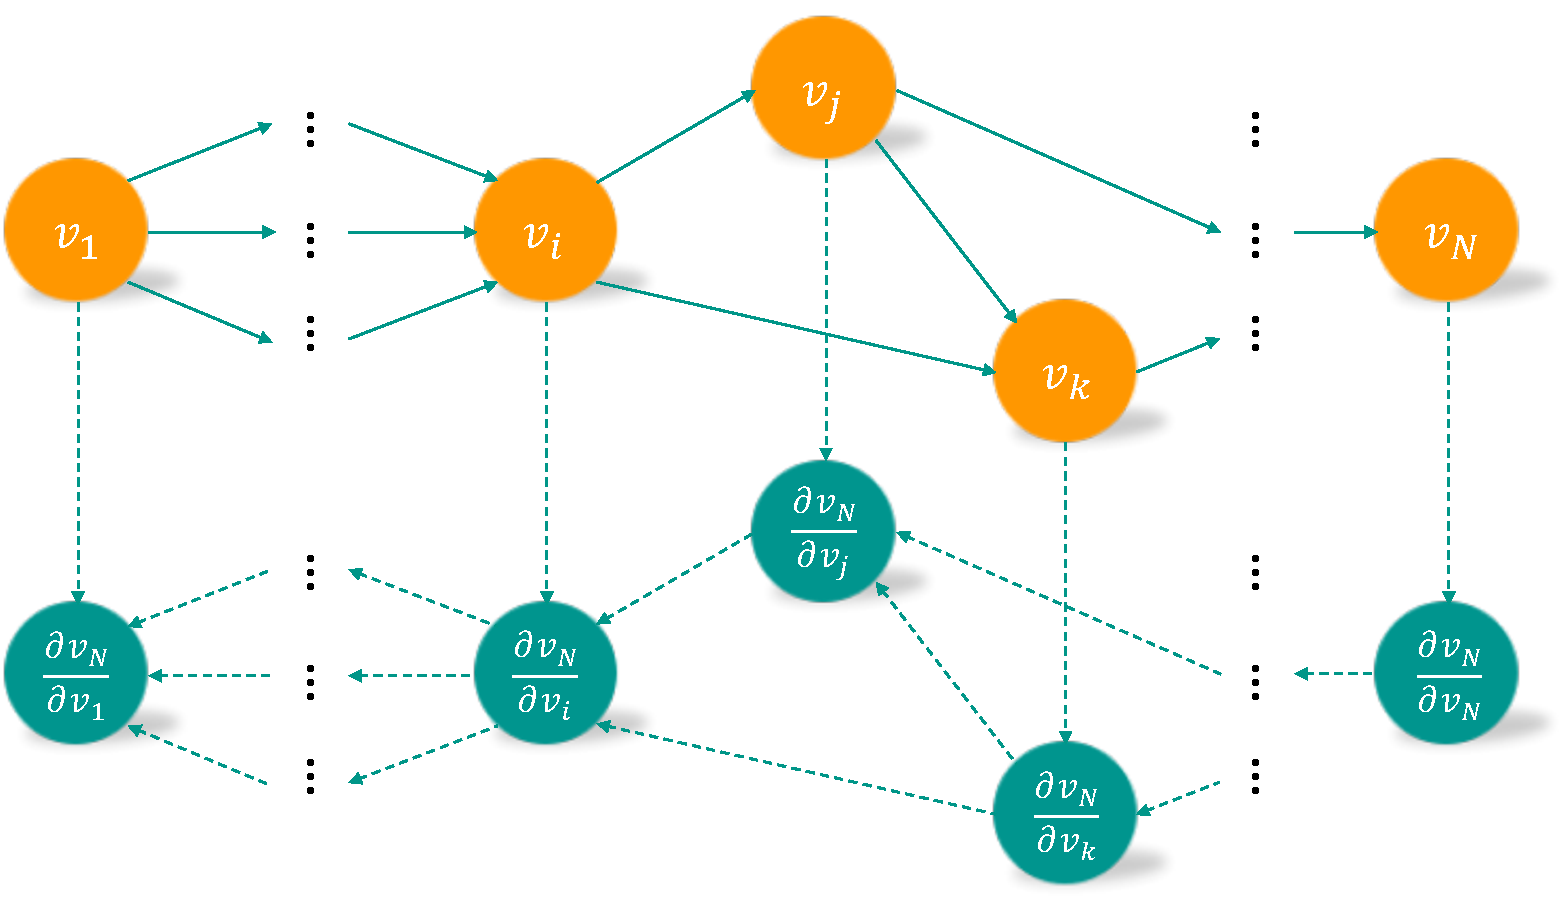
\includegraphics[width=1.0\linewidth]{figures/computational-graph.pdf}
\caption{Demonstration of a directed acyclic computational graph}
\label{fig:dl-dag}
\end{center}
\end{figure}

Suppose all the nodes $v_1,\dots,v_N$ are vectorized and \emph{topologically sorted}, \ie, $(v_i, v_j)\notin E, \forall i < j$. For arbitrary $i < k$, the gradients of node $v_k$ \wrt $v_i$ can be computed by
\begin{equation} \label{eq:grad-dag}
  \frac{\partial v_k}{\partial v_i} = \sum_{j | (v_i, v_j) \in E} \left(\frac{\partial v_j}{\partial v_i}\right)^T \frac{\partial v_k}{\partial v_j},
\end{equation}
where $\partial v_j/\partial v_i$ is informally the Jacobian matrix of $v_j$ \wrt $v_i$.

In neural networks, $v_N$ (and maybe some other nodes that have no outgoing edges) is typically the loss. Thus to compute the gradient of loss \wrt the parameter nodes, we can similarly perform a two-pass computation. In the forward pass (solid arrows in Figure~\ref{fig:dl-dag}), we sequentially compute the values from $v_1$ to $v_N$ and store all their values in temporary buffers. And then in the backward pass (dashed arrows in Figure~\ref{fig:dl-dag}), we compute the gradient of $v_N$ \wrt to each node $v_i$ based on Eq.~\eqref{eq:grad-dag} sequentially from $v_N$ to $v_1$. Whenever a forward or backward node is computed, we can virtually remove all its incoming edges. This would make some nodes no longer have outgoing edges and we can safely reuse their data buffer during implementation to save memory.
% subsection dl-bp-on-graphs (end)





% section dl-bp (end)
